\section{ML Workload Optimizations} \label{sec-ml-workloads}
In this section, we first describe the common types of operations in machine learning workloads.
Then, we discuss how to capture and store the operations in the experiment database.
We also introduce a materialization strategy for only storing the generated data artifacts during the execution of a workload.
Lastly, we discuss how do we utilize the experiment database to optimize new workloads.

\subsection{Operations in ML Workloads}
We assume the main units of work are dataframe (e.g., Pandas, R Data Frames, and Spark DataFrames) like objects that contain one or many columns, where all the data items in one column are of the same data type.
We divide the operations in the ML workloads into 3 categories.
\begin{table}
\centering
\begin{tabular}{ll}
\hline
	   Feature Extraction & Feature Selection\\ \hline
        feature hasher & variance threshold  \\
        one hot encoding & select k best \\
        count vectorizer& select percentile \\ 
        tfidf transformer & recursive feature elimination \\
        hashing vectorizer & select from model \\
        extract\_patch\_2d &  \\
        \hline
\end{tabular}
\caption{List of feature extraction and feature selection operations}\label{feature-engineering-operations}
\end{table}

\subsubsection{Data and Feature Engineering}
This group of operations typically belongs to three categories, i.e., simple data transformations and aggregations, feature selection, and feature extraction.
All of these operations, receive one or multiple columns of a dataset and return another dataset as result. 
While different data processing tools may provide specialized data transformation and aggregation operations for dataframe objects, most of them provide the same or similar operations such as map, reduce, group by, concatenation, and join. 
In Table \ref{feature-engineering-operations}, we show a list of the most common feature extraction and feature selection operations.

\subsubsection{Model Training}
Model training operations are a group of operations that receive a dataset (or one or multiple columns of a dataset) and return a machine learning model.
The result of model training operations can either be used in other data and feature engineering operations (e.g., applying PCA to reduce the number of dimensions of the data) or can be used to perform prediction (for classification and regression tasks) on unseen data.

\subsubsection{Hyperparameter Tuning}
Before training a machine learning model, one has to set the hyperparameters of the model to appropriate values.
Typically, the best values for the hyperparameters of a model vary across different datasets.
The goal of hyperparameter tuning operations is to find the machine learning models with the best performance.
A hyperparameter tuning operation is defined by a budget and a search method.
The budget specifies how many models with different hyperparameter values the operation should train and the search method specifies what search strategy should be incorporated.
We limit our focus to popular search methods, namely, grid search, random search, and Bayesian hyperparameter search \cite{bergstra2012random,snoek2012practical}.

\subsection{Experiment Graph Representation}\label{sub-graph-construction}
To efficiently apply our optimizations, we utilize a graph data structure, called the experiment graph, to store the meta-data and artifacts of the machine learning workloads.
Let $\mathcal{V}=\{v_i\}, i = 1, \cdots, n$ be a collection of artifacts that exist in the workload.
Each artifact is either a raw dataset, a pre-processed dataset resulting from a feature engineering operation, or a model resulting from a model training operation.
Let $\mathcal{E}=\{e_i\}, i = 1, \cdots, m$ be a collection of executed operations that exist in the workload.
A directed edge $e$ from $v_i$ to $v_j$ in $\mathcal{G}(\mathcal{V},\mathcal{E})$ indicates that the artifact $v_j$ is (fully or partially) derived from the artifact $v_i$ by applying the operation in $e$.
Every vertex $v$ has the attribute $\langle s \rangle$ (accessed by $v.s$), which represents the storage size of artifact when materialized.
Every edge $e$ has the attributes $\langle f, t\rangle$ (accessed by $e.f$ and $e.t$), where $f$ represents the frequency of the operation (the number of times the operation has been executed) and $t$ represents the average run-time (in seconds) of the operation.
Each vertex contains meta-data about the artifacts, such as the name and type of the columns for datasets and name, size, the value of parameters and hyperparameters, and the error metric of the models.
Each edge contains the meta-data about the operation, such as the function name, training algorithm, hyperparameters, and in some cases even the source code of the operation.
When a new machine learning workload is executed, we extend the graph to capture the new operations and artifacts.
If an operation already exists in the graph, we update the frequency and average run-time attributes.
Otherwise, we add a new edge and vertex to the experiment graph, representing the new operation and the artifact.
Figure \ref{fig-experiment-graph}a shows an example graph constructed from the code in Listing \ref{listing-experiment-graph}.
To uniquely identify an edge, we utilize a hash function that receives as input the operation and its hyperparameters (if it has any).

\begin{lstlisting}[language=Python, caption=Example script,captionpos=b,label = {listing-experiment-graph}]
import numpy as np
import pandas as pd

from sklearn import svm
from sklearn.feature_selection import SelectKBest
from sklearn.feature_extraction.text import CountVectorizer

train = pd.read_csv('../input/train.csv') 
print train.columns # [ad_desc,ts,u_id,price,y]
vectorizer = CountVectorizer()
count_vectorized = vectorizer.fit_transform(train['ad_desc'])
selector =  SelectKBest(k=2)
top_features = selector.fit_transform(train[['ts','u_id','price']], 
				      train['y'])
X = pd.concat([count_vectorized,top_features], axis = 1)
model = svm.SVC()
model.fit(X, train['y'])
\end{lstlisting}

\begin{figure}
\begin{subfigure}[b]{0.4\linewidth}
\centering
\documentclass{standalone}
\usepackage{tikz}
\usetikzlibrary{graphdrawing, graphs, quotes, positioning,arrows, backgrounds, math, calc, shapes, positioning}
\usegdlibrary{trees}
\begin{document}
\begin{tikzpicture}
%\draw[help lines]  (-2,0) grid (6,6);
\tikzstyle{every node}=[inner sep=0.02cm]
\node (train) [ellipse, draw] at (3,6) {\normalsize $train$};
% layer 1
\node (ad) [ellipse, draw]  at (0,5.5){\normalsize $ad\_desc$};
\node (forselection) [ellipse, draw] at (3.5,5.4) {\normalsize $t\_subset$};
\node (y) [ellipse, draw] at (5.5, 5.5){\normalsize $y$};
% layer 2
\node (cv) [ellipse, draw] at (1,4.9) {\normalsize $cnt\_vect$};
\node(sk) [ellipse, draw]  at (4,4.6){\normalsize $top\_feats$};
% layer 3
%\node (merged1) [circle, draw] at (1.5, 3.5) {$v_6$};
\node (cvsk) [ellipse, draw] at (3.7,3.8) {\normalsize$X$};
% layer 4
%\node(merged2) [circle, draw] at (3, 2.8) {$v_8$};
% layer 5
\node(model) [ellipse, draw, fill=green!20] at (4.9, 3.5)  {$model$};

\graph [grow down,edge quotes ={inner sep=1pt}, edges ={thick},radius=.2cm, nodes={circle, draw,font =\small}]{
(train) [label=train]
->  (ad)
-> (cv)
%-> [anchor=east,align=center,"m"](merged1) 
->(cvsk) 
%-> [anchor=south, align=center,"m"](merged2) ;
-> (model);

(train) 
-> (forselection)
-> (sk)
-> (cvsk) ;

(train) 
->    (y)
%-> [anchor=west, align=center,"m"](merged2) 
->  (model);
};
\end{tikzpicture}
\end{document}
\caption{}
\end{subfigure}%
\begin{subfigure}[b]{0.6\linewidth}
\begin{tabular}{lcl}
\hline
operation & label &  hash \\
\hline
project(ad..) & $\langle 2, 2\rangle$ &p1 \\
project(ts, ..) & $\langle 1, 6\rangle$ & p2\\
project(y) & $\langle 1, 2\rangle$ & p3\\
vectorizer.f\_t & $\langle 2, 40\rangle$ & v1 \\
selector.f\_t & $\langle 1, 60\rangle$ & s1 \\
concat & $\langle 1, 10\rangle$ & c1 \\
merge & $\langle 1, 0 \rangle$ & m\\
model.fit & $\langle 1, 100\rangle$ & f\\
\hline
\end{tabular}
\caption{}
\end{subfigure}
\caption{Experiment graph constructed from the Listing \ref{listing-experiment-graph} (a) and the hash of the operations in the scripts (b)}
\label{fig-experiment-graph}
\end{figure}
Table \ref{fig-experiment-graph}b shows both the label of every edge operation, i.e., frequency and time, and the hash of the operations and their hyperparameters.
We assume the operations project(ad..) and vectorizer.f\_t already exist in the experiment graph.
Therefore, when adding the new operations, we must update their frequency to 2.
In order to represent operations that process multiple input artifacts, e.g., concat and model.fit operations in Listing \ref{listing-experiment-graph}, we proceed as follows.
First, we merge the vertices representing the artifacts into a single vertex using a merge operator.
The merge operator is a logical operator which does not incur a cost, i.e., it has run-time of 0 seconds.
The merged vertex is also a logical vertex with no actual attributes which only contains the vertex id of the merged vertices.
Then, we draw an edge from the merged vertex which represents the actual operation.
For example, in Figure \ref{fig-experiment-graph}a, before applying the concatenation operation, we merge $v_4$ and $v_5$ into $v_6$, then we apply the concatenation operation (c1).
This is a critical step for our materialization algorithm in Section \ref{subsec-materialization} and our optimization strategies discussed in Sections \ref{sec-reuse-and-warmstarting} and \ref{sec-hyperparam-optimization}.

It is important to note that based our definition of a task in Section \ref{sec-introduction} we the workloads belong to multiple different tasks, the constructed graph will contain one connected component for every task.
In the next sections, we assume that the experiment graph contains information about 1 task, although, all the methods described can be applied to multiple tasks as well.

\subsection{Workload Optimization through Experiment Graph}
By utilizing an experiment database, we plan to optimize a new workload by automatically removing redundant operations, speed up the model training, and perform more efficient hyperparameter tuning.

\begin{figure}
\centering
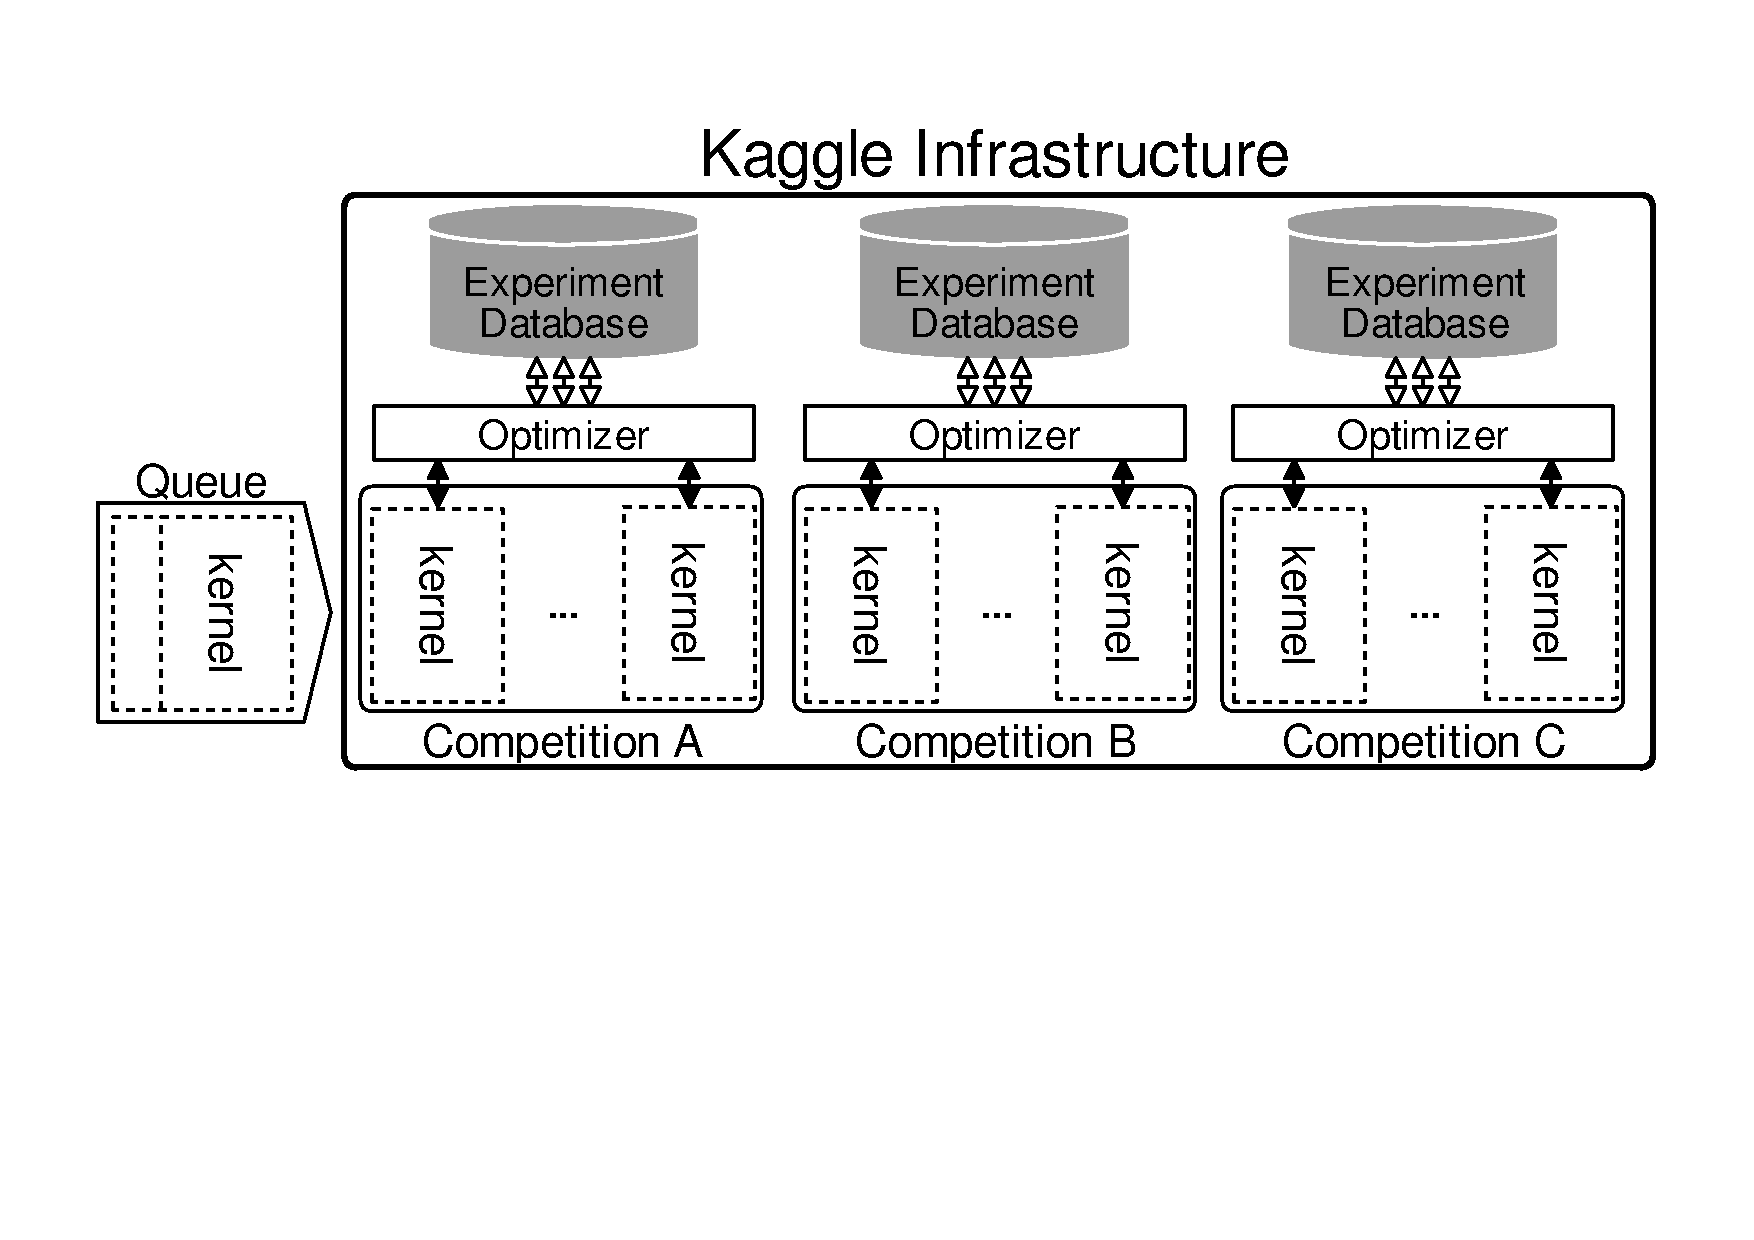
\includegraphics[width=\columnwidth]{../images/improved-use-case}
\caption{Utilizing Experiment Databases in the infrastructure of Kaggle}
\label{improved-use-case}
\end{figure}

Figure \ref{improved-use-case} shows how we utilize the experiment database in the Kaggle Infrastructure. 
The workflow is as follows.
Before executing a kernel (workload), first, an optimizer component analyzes the workload.
Then, the optimizer searches for optimization opportunities by querying the experiment database.
For example, if a new kernel is trying to standardize the dataset or perform a model training, 
the optimizer queries the experiment database to find out if other users have already executed the operations.
Based on the result of the query, the optimizer then decides whether to retrieve the standardized data or the model from the experiment database or execute the operations in the kernel.

In the next sections, we first describe how we utilize the experiment database and what types of optimizations an experiment database enables us to perform.

\todo[inline]{should be merged with previous section}
\subsection{Optimization Workflow}
Figure \ref{fig-system-workflow} shows the workflow of our system.
First, we transform the workload into its graph representation.
Then we utilize the experiment graph to optimize the workload using the techniques in Sections \ref{sec-reuse-and-warmstarting} and \ref{sec-hyperparam-optimization}.
This results in a new workload graph which depending on the types of optimizations may have a fewer number of operations, faster operations, or operation configurations that lead to higher quality machine learning models.
\begin{figure}
\centering
\newcommand*{\connectorH}[4][]{
  \draw[#1, thickarrow] (#3) -| ($(#3) !#2! (#4)$) |- (#4);
}
\begin{tikzpicture}%[background rectangle/.style={fill=olive!45}, show background rectangle]
\tikzstyle{thickarrow}=[line width=0.5mm,draw=gray!128,-triangle 45,postaction={draw, line width=1mm, shorten >=1mm, -}]
\tikzstyle{every label}=[font=\scriptsize]
\tikzstyle{graphnode} = [inner sep=0.04cm, fill=black!255]
\tikzstyle{dummynode} = [inner sep=0.04cm, fill=black!0, line width=0mm]
%\draw[step=1cm,gray,very thin] (-2,0) grid (6,4);

%dummy nodes
\node(dn0) at (0.7, 3) {};
\node(dn1) at (1.7, 3) {};
\node(dn2) at (4.1, 3) {};
\node(dn3) at (5.1, 3) {};
\node(dn4) [inner sep=0.01cm] at (0.3,3) {};

\tikzmath{\x = -1.3; \y =3; }
\node(ws0)[rectangle, text width =1.2cm,minimum width=1.2cm, minimum height=2cm,align=center, draw] at (\x,\y) {workload script};

\tikzmath{\x = .7; \y =3.65; }
\node(wg0)[graphnode,circle, draw] at (\x,\y) {};
\node(wg1)[graphnode,circle, draw] at (\x-0.2,\y-0.4){};
\node(wg2)[graphnode,circle, draw] at (\x-0.2,\y-0.8) {};
\node(wg3)[graphnode,circle, draw] at (\x-0.4,\y-1.2) {};
\node [text width =1.5cm, align=center] at (0.5,2) {original workload};

\tikzmath{\x = 2.9; \y =3.6; }
\node(eg0)[graphnode,circle, draw] at (\x,\y) {};
\node(eg1)[graphnode,circle, draw] at (\x-0.5,\y-0.4) {};
\node(eg2)[graphnode,circle, draw] at (\x,\y-0.4) {};
\node(eg3)[graphnode,circle, draw] at (\x+0.5,\y-0.4) {};
\node(eg4)[graphnode,circle, draw] at (\x -0.75,\y-0.8) {};
\node(eg5)[graphnode,circle, draw] at (\x-0.25,\y-.8){};
\node(eg6)[graphnode,circle, draw] at (\x + 0.25,\y-.8) {};
\node(eg7)[graphnode,circle, draw] at (\x+.75,\y-.8) {};
\node(eg8)[graphnode,circle, draw] at (\x-1,\y-1.2) {};
\node(eg9)[graphnode,circle, draw] at (\x -0.5,\y-1.2) {};
\node(eg10)[graphnode,circle, draw] at (\x,\y-1.2){};
\node(eg11)[graphnode,circle, draw] at (\x + 0.5,\y-1.2) {};
\node(eg12)[graphnode,circle, draw] at (\x+1,\y-1.2) {};
\node [text width =1.5cm, align=center] at (2.9,1.6) {Experiment graph};

\tikzmath{\x = 5.5; \y =3.4; }
\node(og0)[graphnode,circle, draw] at (\x,\y) {};
\node(og1)[graphnode,circle, draw] at (\x-0.2,\y-0.4){};
\node(og2)[graphnode,circle, draw] at (\x-0.4,\y-0.8) {};
\node [text width =1.5cm, align=center] at (5.3,2) {optimized workload};
\draw[dashed, thick] (1.7,2.1) rectangle (4.1,3.9);
\graph []{
(ws0) -> [>=stealth, line width=0.7mm] (dn4);
(wg0) -> (wg1) -> (wg2) -> (wg3);
(eg0) -> (eg1) -> (eg4) -> (eg8);
(eg0) -> (eg2) -> (eg5) -> (eg9);
(eg5) -> (eg10);
(eg0) -> (eg3) -> (eg7) -> (eg12);
(eg3) -> (eg6) -> (eg11);
(eg2) -> (eg6);
(og0) -> (og1) -> (og2);
(dn0) -> [>=stealth, line width=0.7mm] (dn1);
(dn2) -> [>=stealth, line width=0.7mm](dn3);
};
\end{tikzpicture}
\caption{System workflow}
\label{fig-system-workflow}
\end{figure}
